\documentclass{article}

\usepackage{graphics}
\usepackage{graphicx}
\usepackage[a4paper,
            top=2cm,
            bottom=3cm,
            left=3cm,
            right=2cm,
            marginparwidth=1.75cm
            ]{geometry}

\usepackage{float}
\usepackage{subcaption}

\title{TP02 - Estrutura de dados}
\author{Marcos Daniel Souza Netto - 2022069492} 
\date{\today}

\begin{document}
\maketitle

\section{Introdução}

O problema proposto consiste em implementar um programa que recebe um grafo 
e a coloração dos seus vértices e verifica se a coloração dada é gulosa, ou seja,
todo vertíce deve possuir a cor $i$ somente se existir vertices adjacentes
a ele com cores $1, 2, ..., i-1$. Por fim, também deve ser retornada a permutação
dos vértices utilizada na coloração gulosa, isto é, apresentar como o grafo foi 
colorido, apresentando os vértices de cor $i$ seguidos dos vértices de cor $i+1$, 
os vértices de cada cor devem estar ordenados pelo seu rótulo.

A solução implementada leva em consideração a quantidade de vértices mínima de diferentes cores, 
menor que a cor do vértice analisado, para que a coloração seja gulosa. Observe que para satisfazer 
condição de gulosidade é necessário que cada vértice de cor $i$ tenha pelo menos $i-1$ vértices adjacentes 
de cores menores que $i$. Para isso, foi utilizada a estrutura de dados \textbf{set}, tal que para \underline{todo} vértice
de cor menor que $i$, é inserido sua cor no set, e depois de passar por todos essas cores, é verificado se o tamanho do set 
é menor que $i-1$, caso seja, a coloração não é gulosa.

Para a parte da permutação usada, apenas foi utilizada a ordenação escolhida de modo que a comparação entre dois vértices é feita 
pelo sua cor primeiramente, e caso sejam iguais, é feita a comparação pelo seu rótulo.

\section{Método}

A seguir serão detalhados a implementação da solução, de modo a explicitar 
as estruturas de dados utilizadas e as estratégias de solução. A priori vale 
apresentar as especificações do ambiente de desenvolvimento utilizado:

\begin{itemize}
    \item Sistema Operacional: Ubuntu 22.04.3 LTS;
    \item Compilador: G++ 11.4.0;
    \item Processador: Ryzen 5 5500u;
    \item Memória RAM: 8GB.
\end{itemize}


\subsection{Estruturas de dados}

Em síntese, foram utilizadas as seguintes estruturas de dados:

\begin{itemize}
    \item \textbf{set}: Estrutura de dados que armazena elementos únicos, e que permite a inserção, remoção e busca em tempo $O(log(n))$, 
    para tanto ela foi implementada como uma árvore binária de busca, e foi utilizada para armazenar as cores dos vértices adjacentes;    

    \item \textbf{vector}: Estrutura de dados que armazena elementos em sequência contínua de memória. Foi utilizada para representar o grafo, 
    ou seja, o grafo aqui foi representado como um vetor de listas de adjacências, onde cada posição do vetor representa um vértice, tal que cada 
    posição possui um subvetor contendo os vértices adjacentes a ele;

    \item \textbf{pair}: Tipo abstrato de dados que generaliza a ideia de um par ordenado. Foi utilizada para representar a coloração do grafo, 
    o primeiro elemento do par é a coloração do vértice, e o segundo elemento é seu rótulo. Permitiu que a construção da permutação usada na solução seja 
    feita de forma mais simples, pois a ordenação no \emph{vector} de \emph{pairs} é feita pelo primeiro elemento do par, e caso sejam iguais, é feita a ordenação pelo segundo elemento;

\end{itemize}

A implementação dessas estruturas se localizam nos arquivos \emph{set.hpp}, \emph{vector.hpp}, \emph{graph.hpp} e \emph{pair.hpp}.

\subsection{Classes e principais funções}
O código foi dividido nos arquivos já mencionados (\emph{set.hpp}, \emph{vector.hpp}, \emph{graph.hpp} e \emph{pair.hpp}), e também no arquivo \emph{sort.hpp} dos métodos de ordenação implementados e o arquivo principal \emph{main.cpp}.
\begin{itemize}
    \item \textbf{set.hpp}: Implementação da estrutura de dados \emph{set}, por meio de uma árvore binária de busca não balanceada, que foi utilizada para armazenar as cores dos vértices adjacentes. Foram implementados os principais métodos da estrutura, como: \emph{insert}, \emph{remove}, \emph{find}, \emph{getSize}, \emph{walk} e \emph{clear};
        \subitem \textbf{walk}: Percorre o \emph{set}, e para cada elemento, chama uma função passada como parâmetro;

    \item \textbf{vector.hpp}: Implementação da estrutura de dados \emph{vector}, um array de memória contíguo como tamanho podendo ser aumentado e controlado pela própria estrutura. Foram implementadas as principais funções da estrutura, como: \emph{push\_back}, \emph{pop\_back}, \emph{insert},  \emph{getSize};

    \item \textbf{sort.hpp}: Implementação dos métodos de ordenação utilizados.
        \subitem \textbf{bubleSort}: Consiste em percorrer o vetor, e para cada elemento, percorrer o vetor novamente, e caso o elemento atual seja maior que o próximo, eles são trocados de posição;
        \subitem \textbf{insertionSort}: Consiste em percorrer o vetor, e para cada elemento inseri-lo na posição correta do subvetor ordenado;
        \subitem \textbf{selectionSort}: Consiste em percorrer o vetor, e para cada elemento, percorrer o subvetor não ordenado, e encontrar o menor elemento, e trocá-lo de posição com o elemento atual;
        \subitem \textbf{mergeSort}: Consiste em dividir o vetor em dois subvetores, ordenar cada um deles e depois juntá-los de forma ordenada;
        \subitem \textbf{quickSort}: Consiste em escolher um pivô, e colocar todos os elementos menores que ele a sua esquerda, e todos os elementos maiores que ele a sua direita, e depois ordenar recursivamente os subvetores a esquerda e a direita da partição criada;
        \subitem \textbf{heapSort}: Consiste em construir uma \emph{heap} a partir do vetor, e depois retirar o elemento do topo da \emph{heap} e colocá-lo no final do vetor, e repetir esse processo até que a heap esteja vazia;
        \subitem \textbf{swap}: Função que troca dois elementos de posição no vetor;
    
    \item \textbf{pair.hpp}: Tipo abstrato de dados de par ordenado, com os elementos \emph{first} e \emph{second}. Foi implementadas as funções de comparação específicas para o problema proposto (Comparação pelo primeiro elemento, e caso sejam iguais, comparação pelo segundo elemento);
    \item \textbf{graph.hpp}: Tipo abstrato de dados que representa um grafo por uma lista de adjacência utilizando a estrutura \emph{vector}. 
    \item \textbf{main.cpp}: Arquivo principal do programa, onde é feita a leitura da entrada, e a chamada das funções que resolvem o problema proposto.
        \subitem \textbf{sort}: Função que recebe um vetor de \emph{pairs} e um método de ordenação, e ordena o vetor utilizando o método de ordenação passado como parâmetro;
        \subitem \textbf{verifyGreedy}: Função que recebe um grafo e uma coloração, e verifica se a coloração é gulosa, retornando \emph{true} caso seja, e \emph{false} caso contrário;
    
\end{itemize}

\section{Análise de Complexidade}

A seguir serão apresentadas as análises de complexidade das principais funções do programa.

\subsection{infixToPosfix}
Como mencionado acima, esta função converte uma expressão infixa para a representação posfixa. Para isso, a função percorre a string contendo a expressão infixa, e para cada caractere, verifica se ele é um operando ou um operador. Caso seja um operando, ele é adicionado à string de saída, caso seja um operador, ele é adicionado à pilha. Ao final da leitura da string, todos os operadores que estão na pilha são adicionados à string de saída. Portanto, a complexidade da função é $O(n)$, onde $n$ é o tamanho da string de entrada.

A complexidade de espaço é $O(n)$, pois a pilha pode conter no máximo $n$ elementos.

\subsection{evaluateExpression}
Esta função recebe um vetor de inteiros representando a expressão booleana na forma posfixa e um vetor contendo os valores das variáveis da expressão e retorna o resultado da expressão. Para isso, a função percorre esse vetor de entrada, e para cada elemento, verifica se ele é um operando ou um operador (inteiros negativos). Caso seja um operando, ele é adicionado à pilha, caso seja um operador, ele é removido dois operandos do topo da pilha ou apenas um operando (No caso do operador $\sim$), e o resultado da operação é adicionado à pilha. Ao final da leitura da string, o resultado da expressão é o elemento que está no topo da pilha. Portanto, a complexidade da função é $O(n)$, onde $n$ é o número de elementos do vetor de entrada.

A complexidade de espaço é $O(n)$, pois assim como a função anterior, a pilha pode conter no máximo $n$ elementos.

\subsection{satTree}
Esta função recebe um vetor de inteiros representando uma expressão booleana na forma posfixa, um vetor contendo os valores das variáveis da expressão(agora podendo conter quantificadores existe e para todo) e retorna 1 ou 0 caso a expressão seja satisfazível ou não, respectivamente. Caso ela seja satisfazível, uma string contendo a possível solução é retornada. 

Para isso, a função indexa os quantificadores da expressão, em seguida percorre o vetor dos quantificadores construindo a árvore de solução pelos últimos quantificadores até o primeiro.
A árvore possui, portanto, como folhas os possíveis valores para os quantificadores (0 ou 1) e desse modo ela possui $2^k$ folhas, onde $k$ é o número de quantificadores, seja existe ou para todo. Para exemplificar considere a figura.

% \begin{figure}[H]
%     \centering
%     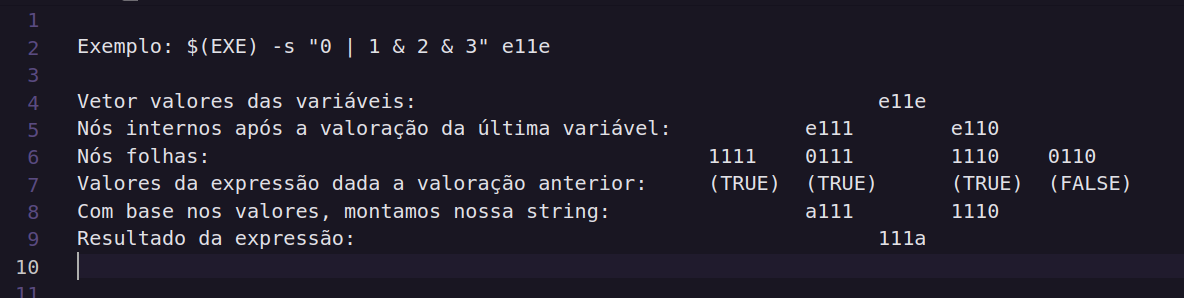
\includegraphics[width=\textwidth]{./images/sat_tree.png}
%     \caption{Árvore de solução para a expressão $\exists a \exists d , b = c = 1,  (a \lor b \land c \land d)$}
%     \label{fig:sat_tree}
% \end{figure}

Como visto, a árvore possui $2^k$ folhas, e para cada uma delas, a função \textit{evaluatePostfix} é chamada para verificar se a expressão é satisfazível. Portanto, a complexidade da função é $O(2^k)$, onde $k$ é o número de quantificadores.

Já a complexidade de espaço é $O(k)$, pois a solução da árvore é realizada de modo ir o mais profundo na árvore possível, e cada vez que um nó é resolvido, seus filhos são removidos da memória.
\section{Estratégias de robustez}

A estratégia de robustez utilizada foi basicamente a verificação da entrada do usuário, ou seja a verificação na quantidade de argumentos e seus tipos.

\section{Análise Experimental}

A seguir serão apresentados os resultados obtidos na experimentação do programa.

\subsection{Localidade de Referência}

Utilizando o programa analisamem, fornecido pelo professor, foi possível observar a localidade de referência do programa. Importante notar que aqui serão apresentadas imagens relacionadas a parte de satisfatibilidade do programa, afinal utiliza a parte de solucionador de equaações booleanas como subrotina.


Ademais, foi utilizada a seguinte expressão para a parte de satisfatibilidade:

\verb# ./bin/tp01 -s "0 | 1 & 2 & 3" e11e#

% \begin{figure}[H]
%     \centering
%     \hfill
%     \begin{subfigure}[c]{0.4\textwidth}
%         \centering
%         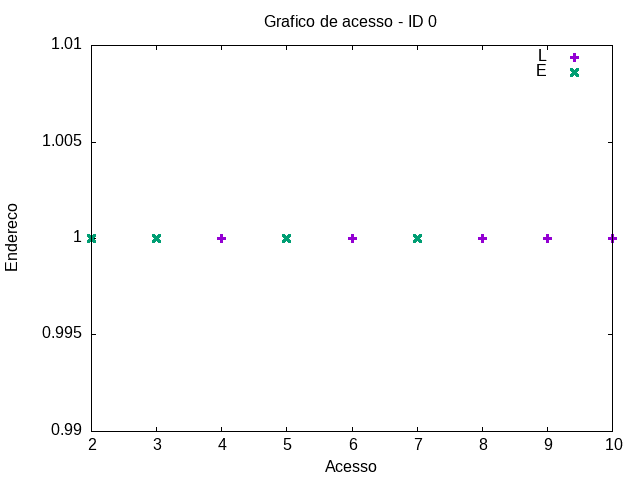
\includegraphics[width=\textwidth]{./images/sat_tree/registro_s-acesso-0.png}
%         \caption{Pilha da função infixToPostfix}
%         \label{fig:ac01}
%     \end{subfigure}%
%     \hfill
%     \begin{subfigure}[c]{0.4\linewidth}
        
%         \centering
%         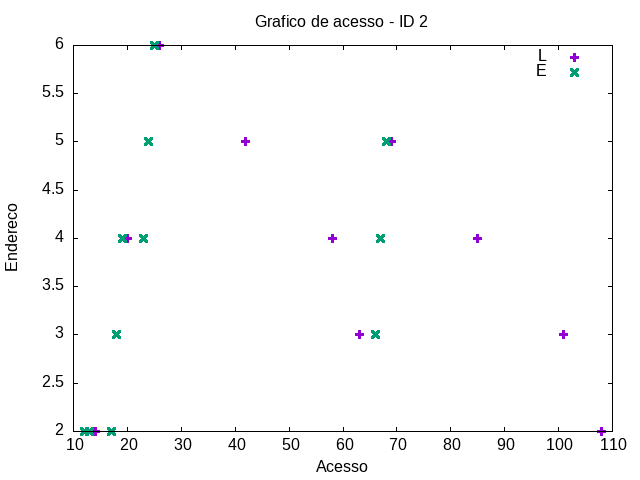
\includegraphics[width=\textwidth]{./images/sat_tree/registro_s-acesso-2.png}
%         \caption{Pilha da função sat\_tree}
%         \label{fig:ac02}
%     \end{subfigure}
%     \hfill
%     \caption{Acesso de Memória}
% \end{figure}

% \begin{figure}[H]
%     \centering
%     \hfill
%     \begin{subfigure}[c]{0.4\textwidth}
%         \centering
%         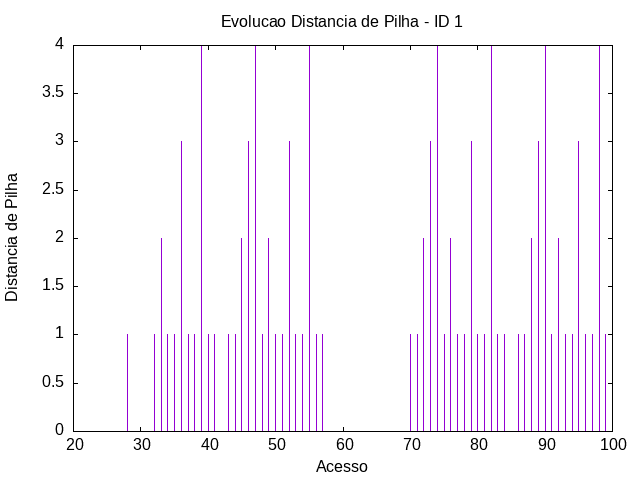
\includegraphics[width=\textwidth]{./images/sat_tree/registro_s-distp-1.png}
%         \caption{Pilha da função evaluateExpression}
%         \label{fig:ac03}
%     \end{subfigure}
%     \hfill
%     \begin{subfigure}[c]{0.4\textwidth}
%         \centering
%         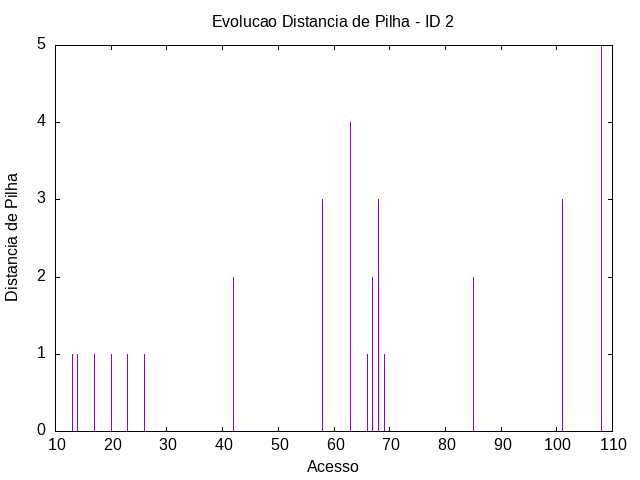
\includegraphics[width=\textwidth]{./images/sat_tree/registro_s-distp-2.png}
%         \caption{Pilha da função sat\_tree}
%         \label{fig:ac04}
%     \end{subfigure}
%     \hfill
%     \caption{Evolução de distância da pilha}
% \end{figure}

% Observa-se nessa Figura 3 (a) que ocorre um padrão em 4 partes, isso se deve porque a função \emph{evaluateExpression} é chamada uma vez para folha da árvore. 
% Outro detalhe sobre a Figura 3 (b) é a possibilidade de observar que o caminhamento na árvore é realizada semelhante a DFS(\emph{Depht First Search}), consonante com a implementação da função \emph{sat\_tree}.

% \begin{figure}[H]
%     \centering
%     \hfill
%     \begin{subfigure}[c]{0.4\textwidth}
%         \centering
%         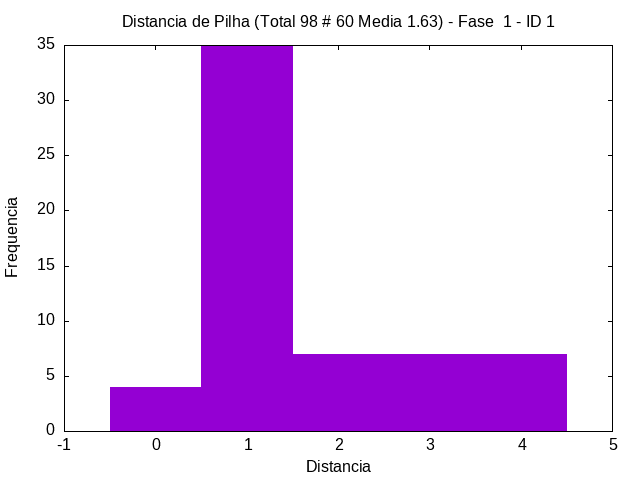
\includegraphics[width=\textwidth]{./images/sat_tree/registro_s-hist-1-1.png}
%         \caption{Pilha da função evaluateExpression}
%         \label{fig:ac05}
%     \end{subfigure}
%     \hfill
%     \begin{subfigure}[c]{0.4\textwidth}
%         \centering
%         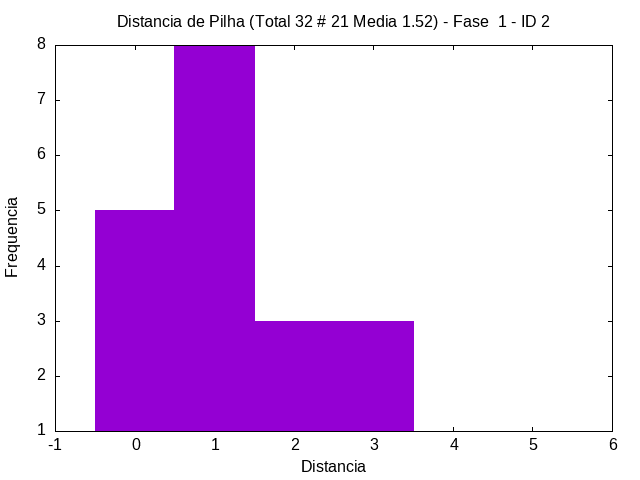
\includegraphics[width=\textwidth]{./images/sat_tree/registro_s-hist-1-2.png}
%         \caption{Pilha da função sat\_tree}
%         \label{fig:ac06}
%     \end{subfigure}
%     \hfill
%     \caption{Distância da pilha}
% \end{figure}

\subsection{Tempo de execução}

Nesse experimento foi realizado medições de tempo de execução a parte de satisfatibilidade do programa, variando o número de quantificadores da expressão. Para isso,
variamos a quantidade de quantificadores da expressão de 13 até 20, para que possamos observar o comportamento do programa para um número maior de quantificadores.
Teve como base o seguinte comando (Atente-se que estamos variando o número de quantificadores): 


\verb#bin/tp01 -s "0 | 1 | 2 | (...) | 17 | 18 | 19" eeeeeeeeeeeeeeeeeeee#

% \begin{figure}[H]
%     \centering
%     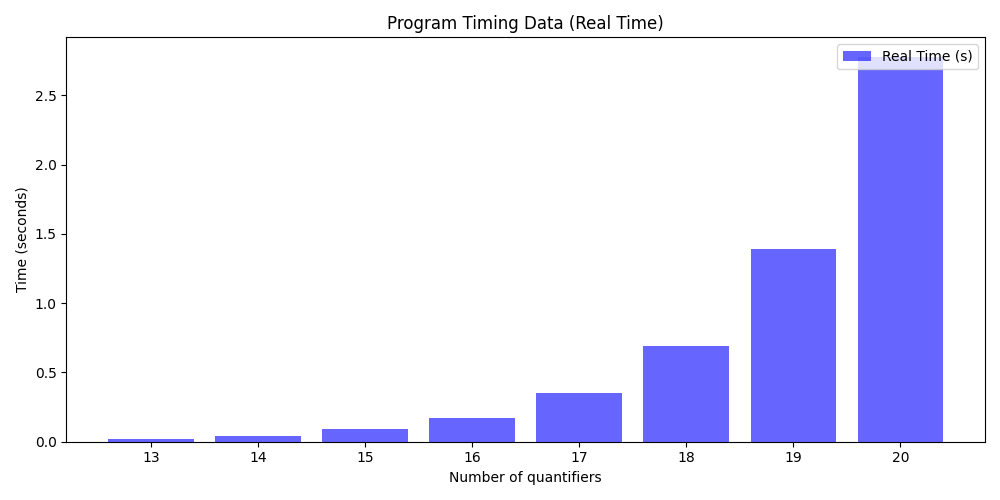
\includegraphics[width=0.6\textwidth]{./images/time.png}
%     \caption{Tempo de execução do programa para diferentes números de quantificadores}
%     \label{fig:time}
% \end{figure}


Observa-se, portanto, comportamento semelhando a ordem de complexidade descrita anteriormente ($O(2^k)$), onde $k$ é o número de quantificadores.

\section{Conclusões}

O trabalho proposto foi de grande valia para o aprendizado de estruturas de dados, e de como elas podem ser utilizadas para solucionar problemas, afinal foi de extrema importância a utilização de pilhas e árvores como estruturas principais.  

Além disso, podemos observar que a análise de complexidade de grande importância, uma vez que ela nos permite prever o comportamento do programa para diferentes entradas, e assim, podemos realizar otimizações no código, como por exemplo, a utilização de uma estrutura de dados mais eficiente. Nesse trabalho, por exemplo, o problema de satisfatibilidade é um problema NP (determinístico não polinomial), ou seja, não existe uma solução conhecida em tempo polinomial, o que condiz com a solução implementada (de complexidade exponencial).

Por fim, a análise do tempo de execução de forma experimental foi de fato interessante pois permitiu conferir a similaridade com a teoria e o mundo real.
\section*{Bibliografia}

Slides da disciplina de Estrutura de Dados, ministrada pelo Prof. Wagner Meira Jr. e Prof. Eder Fereira Figuiredo.


\section*{Instruções para compilação e execução}

Em um terminal, navegue até a pasta raiz do projeto e execute os seguintes comandos:

\begin{verbatim}
    $ make
    $ ./bin/tp1.out -a "<expressão booleana>" <valores das variáveis> // Valor 
    $ ./bin/tp1.out -s "<expressão booleana>" <valores das variáveis> // SAT
\end{verbatim}

\end{document}